\documentclass[24pt]{article}
\usepackage{graphicx} % Required for inserting images
\usepackage{xcolor} % Load the xcolor package
\usepackage{amsmath} % Math symbols
\usepackage{hyperref} % Style hyperreferences
\usepackage{blindtext}
\usepackage{fancyhdr}
\usepackage{subcaption}
\usepackage [ a4paper , margin=1in ] { geometry }
\hypersetup{
    colorlinks=true,
    linkcolor=blue,
    filecolor=magenta,      
    urlcolor=cyan,
}


\title{Enhancing Reasoning Path Diversity in Commonsense Question Answering}
\author{
  Sagnik Nandi\\
  \texttt{23B0905}
  \and
  Harshil Solanki\\
  \texttt{23B1016}
}
\date{}

\begin{document}

\maketitle
\tableofcontents
\clearpage


% \section{Dataset Name: CommonsenseQA (CSQA)}
% \noindent
% \textbf{Dataset:} \url{https://paperswithcode.com/dataset/commonsenseqa}

\section{Paper Overview}

\url{https://arxiv.org/pdf/2203.11171v4}\\ \\
\textbf{Paper Title:}
Self-Consistency Improves Chain of Thought Reasoning in Language Models\\

\noindent The paper investigates methods to enhance the accuracy and performance of Large Language Models (LLMs) through optimized techniques and decoding strategies.
\subsection{Key Techniques Highlighted:}
    \begin{itemize}
        \item \textbf{Chain-of-Thought (CoT) Prompting:} This involves providing illustrative examples to guide the model's reasoning process.
        \item \textbf{Self-Consistency Decoding:} This method generates diverse reasoning paths and selects the most consistent final answer by marginalizing over them.
        \item CoT and self-consistency are effective for tasks with fixed answer sets and can be adapted for open-text generation using suitable consistency metrics.
    \end{itemize}
\subsection{Model Architectures used:}
    \begin{itemize}
        \item \textbf{Decoder-Only Models (e.g., GPT-3, PaLM, LaMDA):}
        \begin{itemize}
            \item Well-suited for autoregressive text generation tasks like conversational AI and creative writing.
            \item Offer simpler architecture and faster inference times.
        \end{itemize}
        \item \textbf{Encoder-Decoder Models (e.g., T5, BART):}
        \begin{itemize}
            \item Better suited for sequence-to-sequence tasks such as translation and summarization.
            \item Provide stronger input-output alignment but with higher computational demands.
        \end{itemize}
    \end{itemize}
\subsection{Sampling Strategies and Self-Consistency:}
    \begin{itemize}
        \item Sampling techniques (e.g., temperature sampling, top-k truncation) are crucial for generating diverse reasoning paths.
        \item Self-consistency decoding outperforms traditional methods like sample-and-rank and beam search in terms of accuracy.
        \item Self-consistency incurs higher computational costs.
        \item The authors suggest using a limited number of reasoning paths to balance performance and efficiency.
    \end{itemize}
\subsection{Limitations and Future Directions:}
    \begin{itemize}
        \item Self-consistency requires significant computational resources.
        \item Self-consistency may generate nonsensical reasoning paths.
        \item Future work could focus on fine-tuning models with supervised data generated through self-consistency to improve single-inference accuracy.
        \item Grounding models' rationale generation remains an open challenge requiring further research for logical and accurate outputs.
    \end{itemize}




\section{Model Overview}
\subsection{Dataset}
\url{https://paperswithcode.com/dataset/commonsenseqa}\\ \\
\textbf{CommonsenseQA} is a new multiple-choice question answering dataset that requires different types of commonsense knowledge to predict the correct answers . It contains 12,102 questions with one correct answer and four distractor answers.

\subsection{Pre-trained LLM}
We are using the \textit{together.ai} interface to prompt with SOTA Language models like \textbf{Llama 4} and \textbf{Deepseek R1}. 

\subsection{Sampling}
It first samples a diverse set of reasoning paths instead of only taking the greedy one, and then selects the most consistent answer by marginalizing out the sampled reasoning paths. Self-consistency leverages the intuition that a complex reasoning problem typically admits multiple different ways of thinking leading to its unique correct answer.

% \textbf{Input:} Data, pretrained language models (like BERT, T5). \\

\subsection{Output} Comparison of the self-consistency method with greedy decoding and other baseline methods (e.g., beam search) to highlight its advantages.


\section{Current Progress and Code}
\subsection{Analysis of Strategies}
\begin{figure}[h]
    \centering
    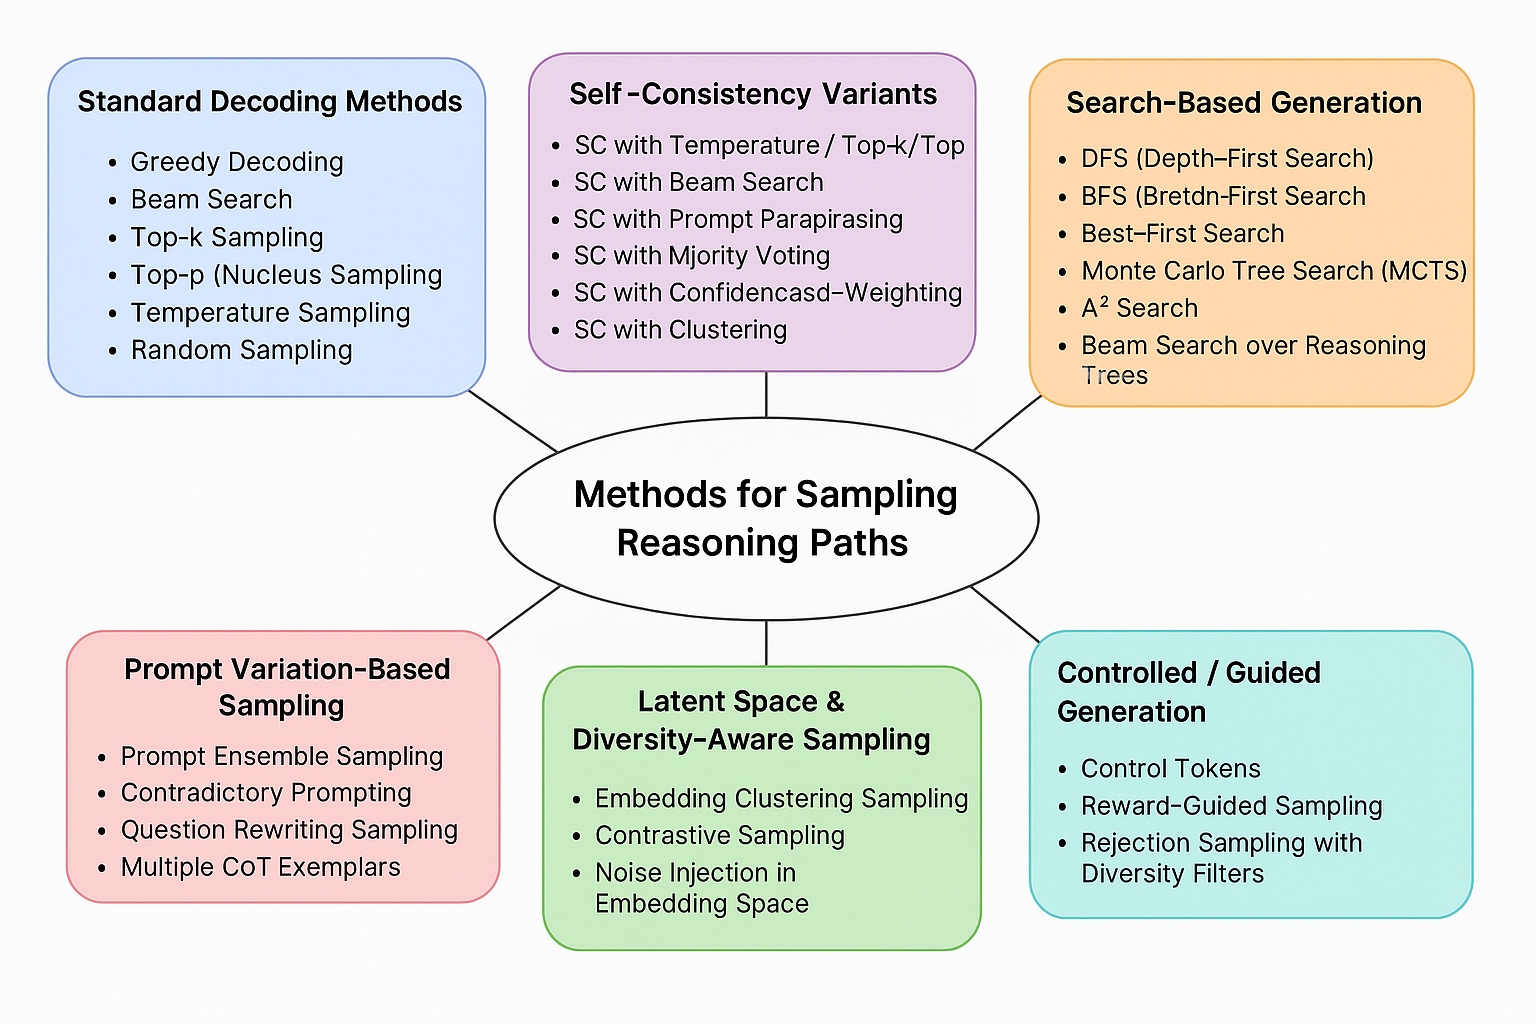
\includegraphics[width=0.8\textwidth]{diagram.png}
    \caption{Different Strategies for Sampling}
    \label{}
\end{figure}
    
\subsection{Dataset Analysis}
An example of 'train' looks as follows:
\begin{verbatim}
{
  `id': `075e483d21c29a511267ef62bedc0461',
  `question': `The sanctions against the school were a punishing blow, and they seemed to _____ 
  the efforts the school had made to change?',
  `question_concept': `punishing',
  `choices': {
    `label': [`A', `B', `C', `D', `E'],
    `text': [`ignore', `enforce', `authoritarian', `yell at', `avoid']
  },
  `answerKey': `A'
}
\end{verbatim}


\subsection{Self-consistency Implementation} 
\begin{itemize}
    \item Ran initial experiments using multiple reasoning paths and beam search
    \item Choose the most common answer based on 10 responses generated, look at \texttt{sc\_10\_samples.py} in self\_implementation
\end{itemize}

\noindent
Github Link : \url{https://github.com/HARSHIL2836R/ReasoningLLMs/tree/main/self_implementation}\\



% \textbf{Source Code:} \url{https://github.com/codelion/optillm/blob/main/optillm/self_consistency.py}\\
% \textbf{Dataset:} \url{https://paperswithcode.com/dataset/commonsenseqa}

\section{Future Plan of Action}

\subsection{Metrics}
Provide metrics like:
\begin{itemize}
    \item Number of unique reasoning paths.
    \item Path similarity measures (e.g., cosine similarity).
    \item Diversity scores (e.g., Shannon entropy) to assess the diversity of generated reasoning paths.
\end{itemize}


\subsection{Strategies}
Basic strategies:
\begin{itemize}
    \item Sample multiple reasoning paths by \textbf{varying temperature} and aggregate answers via majority voting
    \item \textbf{Cluster} the sampled responses based on cosine similarity and select most common answer
\end{itemize}
Advanced strategies:
\begin{itemize}
    \item Generate different paths by \textbf{varying prompts} like paraphrasing the question
    \item Model reasoning steps as a graph and use search strategies like \textbf{BFS}, \textbf{DFS} or \textbf{A*} to discover paths
\end{itemize}

\subsection{Timeline}
\begin{itemize}
    \item \textbf{April 14–20}: Implement basic strategies and different metric computations and compare their performances
    \item \textbf{April 29-30}: Implement advanced strategies and improving the performance
    \item \textbf{May 1–3}: Final analysis, report writing, and polishing of visualizations and results
\end{itemize}

\section{Code References}
\begin{enumerate}
    \item \textbf{Codebase:} \url{https://github.com/codelion/optillm/blob/main/optillm/self_consistency.py}
    \item Drive Link : \url{https://drive.google.com/drive/folders/1Vzzdk7ZRTuls8XM_-3UT0aqaiBEoyV4T?usp=sharing}
\end{enumerate}

\end{document}